\documentclass[reportComp]{thesis}
\usepackage[cpp,linenum]{mypackage}

\title{数值计算方法实验报告}
\subtitle{实验三:最小二乘法}
\school{数据科学与计算机学院}
\author{陈鸿峥}
\classname{17大数据与人工智能}
\stunum{17341015}
\headercontext{数值计算方法实验报告}

\begin{document}

\maketitle

\section{实验题目}
拟合形如$f(x)\approx\dfrac{a+bx}{1+cx}$的函数的一种快速方法是将最小二乘法用于下列问题:$f(x)(1+cx)\approx a+bx$,试用这方法拟合下表给出的中国人口数据。
\begin{center}
\begin{tabular}{ccc}\hline
次序 & 年份 & 人口(亿)\\\hline
第一次 & 1953 & 5.82 \\
第二次 & 1964 & 6.95 \\
第三次 & 1982 & 10.08 \\
第四次 & 1990 & 11.34 \\
第五次 & 2000 & 12.66 \\\hline
\end{tabular}
\end{center}

通过图形来展示拟合效果。

\section{实验目的}
理解最小二乘法的原理并应用到实际生活中。

\section{实验原理与内容}
% 若有推导的式子,写在这里
% 重要代码和截图
将方程$f(x)(1+cx)\approx a+bx$改写为
\[f(x)\approx a+bx-cxf(x)\]
因此可看作基函数为
\[\phi_0(x)=1,\;\phi_1(x)=x,\;\phi_2(x)=-xf(x)\]
设$\vx=\bmat{x_1 & \cdots & x_5}^\T$进而
\[\bmat{\phi_0(\vx) & \phi_1(\vx) & \phi_2(\vx)}\bmat{a\\b\\c}=f(\vx)\]
即可解得$a,b,c$。
或通过解法方程
\[\bmat{\lrang{\phi_0,\phi_0} & \lrang{\phi_0,\phi_1} & \lrang{\phi_0,\phi_2}\\\lrang{\phi_1,\phi_0} & \lrang{\phi_1,\phi_1} & \lrang{\phi_1,\phi_2}\\\lrang{\phi_2,\phi_0} & \lrang{\phi_2,\phi_1} & \lrang{\phi_2,\phi_2}}\bmat{a\\b\\c}=\bmat{\lrang{f,\phi_0}\\\lrang{f,\phi_1}\\\lrang{f,\phi_2}}\]
也可得到$a,b,c$。

下面为本次实验的Mathematica源代码,\textbf{用两种方法求解},完整文件已在附件中\verb'LeastSquares.nb'。
\begin{lstlisting}[language=mathematica]
x = {1953, 1964, 1982, 1990, 2000};
y = {5.82, 6.95, 10.08, 11.34, 12.66};
\[Phi]0 = ConstantArray[1, 5];
\[Phi]1 = x;
\[Phi]2 = Table[-x[[i]]*y[[i]], {i, 1, 5}];
A = Transpose[{\[Phi]0, \[Phi]1, \[Phi]2}];
LeastSquares[A, y](*Inner function*)
(*My implementation below*)
\[Phi][i_, x_] := 
 If[i == 0, \[Phi]0[[x]], 
  If[i == 1, \[Phi]1[[x]], If[i == 2, \[Phi]2[[x]]]]]
A = Table[
   Table[Sum[\[Phi][i, k]*\[Phi][j, k], {k, 1, 5}], {j, 0, 2}], {i, 0,
     2}];
b = Table[Sum[\[Phi][i, k]*y[[k]], {k, 1, 5}], {i, 0, 2}];
result = Inverse[A].b
Show[ListPlot[Table[{x[[i]], y[[i]]}, {i, 1, 5}]], 
 Plot[(result[[1]] + result[[2]] k)/(result[[3]] k + 1), {k, 1950, 
   2010}], AxesLabel -> {HoldForm[Year], HoldForm[Population]}]
\end{lstlisting}

\section{实验结果与分析}
% 对运行结果说明(图像截图,数据列成表)并分析
两种方法求解出来的结果相同,均为
\[\begin{cases}
a=2.94562\\
b=-0.00140662\\
c=-0.000495599
\end{cases}\]
拟合结果如图~\ref{fig:res}所示。
\begin{figure}[H]
\centering
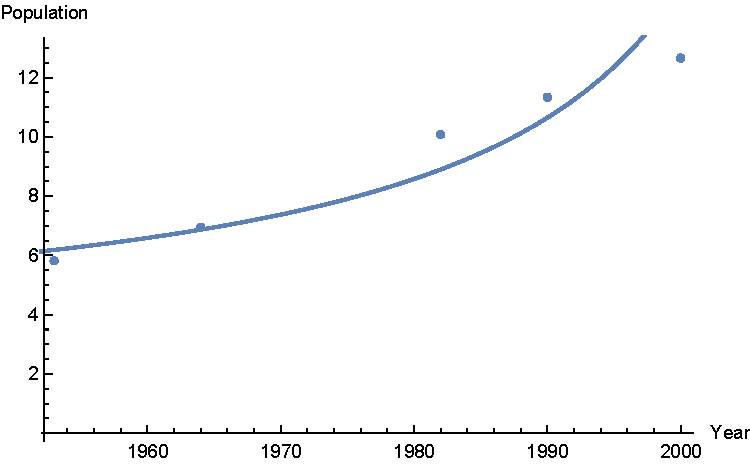
\includegraphics[width=0.5\linewidth]{result.pdf}
\caption{拟合结果}
\label{fig:res}
\end{figure}

\section{实验总结和心得}
本次实验熟悉了最小二乘法的原理,并用两种方法实施求解,收获良多。

\end{document}
% 1024180018@qq.com
% shuzhijisuan2017@163.com

% ftp://172.18.216.222
% shuzhi2019
% 学号_姓名_weekX_vY

% 上机作业要求
% 建议使用C++/Matlab编程,注:不允许使用内置函数完成主要功能
% 主题/文件名:班级+姓名(小组)+学号+第几次作业
% 实验报告(运行结果)、源代码